\documentclass[UTF8,a4paper,11pt]{article}
\usepackage{ctex}

\usepackage{mathtools}
\usepackage{amsmath}
\usepackage{amsfonts}
\usepackage{amssymb}
\usepackage{amsthm}
\usepackage[T1]{fontenc}
\usepackage{indentfirst}

\usepackage{graphicx}
\usepackage{geometry}
\usepackage{latexsym}
\usepackage{fancyhdr}
\usepackage{titlesec}
\usepackage{setspace}
\usepackage{enumerate}
\usepackage{enumitem}
\usepackage{multicol}
\usepackage{url}
\usepackage{ulem}
\usepackage{bm}
\usepackage{hyperref}
\usepackage{stfloats}

\setlength{\parindent}{2em}
\linespread{1.2}
\usepackage{listings}
\usepackage{xcolor}
\usepackage{algorithm}
\usepackage{algorithmicx}
\usepackage{algpseudocode}
\usepackage{mdframed}
\usepackage{booktabs}
\usepackage{multirow}
\usepackage{float}
\usepackage{makecell}

\everymath{\displaystyle}

\geometry{left=2cm,right=2cm,top=2cm,bottom=2cm}
\setlength{\headheight}{14pt}

\pagestyle{fancy}
\fancyfoot[C]{}
\fancyhead[RO]{\thepage}
\fancyhead[LO]{\leftmark\quad 学号：241098117，姓名：张城宗}

\titleformat{\section}{\bfseries\Large}{$\S$\,\thesection\,}{1em}{}
\setenumerate[1]{itemsep=0pt,partopsep=0pt,parsep=\parskip,topsep=0pt}
\setitemize[1]{itemsep=0pt,partopsep=0pt,parsep=\parskip,topsep=0pt}

\newcommand*{\rmk}{\textbf{注：}}
\newcommand\e{\leftarrow}

% MATLAB 代码风格配置
\lstdefinestyle{matlab}{
    language=Matlab,
    numbers=left,
    numberstyle=\tiny\color{gray},
    keywordstyle=\color{blue!80!black},
    commentstyle=\color{green!50!black},
    stringstyle=\color{orange!80!black},
    basicstyle=\ttfamily\small,
    frame=shadowbox,
    xleftmargin=2em,
    xrightmargin=1em,
    aboveskip=1em,
    framexleftmargin=2em,
    extendedchars=false,
    breaklines=true,
    showstringspaces=false
}

\begin{document}

\begin{center}
{\huge \textbf{数值分析第二周上机作业}}

\vspace{0.3cm}
{\large 学号：241098117\quad，姓名：张城宗\quad}
\end{center}

\section{问题描述}

对 Runge 函数
$$R(x) = \frac{1}{1+x^2}, \quad x \in [-5,\,5],$$
分别用以下五种插值方法逼近，绘图比较各方法的逼近效果，并分析误差：

\begin{enumerate}
  \item 等距节点 Newton 插值多项式（10 次，11 个节点）；
  \item Chebyshev 节点 Lagrange 插值多项式（20 次，21 个节点）；
  \item 等距节点分段线性插值（11 个节点）；
  \item 等距节点三次样条插值（11 个节点，not-a-knot 边界条件）；
  \item 等距节点分段三次 Hermite 插值 PCHIP（11 个节点）．
\end{enumerate}

\section{数值方法与算法思路}

\subsection{方法（1）：等距节点 Newton 插值（10 次）}

\noindent\textbf{Newton 插值公式．}
Newton 插值多项式利用均差（divided difference）构造，形式为
$$N_n(x) = f[x_0] + f[x_0,x_1](x-x_0) + f[x_0,x_1,x_2](x-x_0)(x-x_1) + \cdots + f[x_0,\ldots,x_n]\prod_{k=0}^{n-1}(x-x_k).$$

均差的递推定义为
$$f[x_k,\ldots,x_{k+j}] = \frac{f[x_{k+1},\ldots,x_{k+j}] - f[x_k,\ldots,x_{k+j-1}]}{x_{k+j} - x_k}.$$

\noindent\textbf{Runge 现象．}
对 $R(x)$ 在 $[-5,5]$ 取 11 个等距节点（$x_k = -5+k,\ k=0,1,\ldots,10$）做 10 次多项式插值，插值多项式在端点 $x=\pm5$ 附近会产生剧烈振荡，误差不随次数增大而减小，甚至发散．这是因为等距节点的节点多项式 $\omega_{n+1}(x) = \prod_{k=0}^{n}(x-x_k)$ 在端点附近取值极大．

\noindent\textbf{Horner 嵌套求值（秦九韶算法）．}
将 Newton 插值多项式改写为嵌套形式从最高阶开始计算：
$$N_n(x) = \bigl(\cdots\bigl((c_n(x-x_{n-1}) + c_{n-1})(x-x_{n-2}) + c_{n-2}\bigr)\cdots\bigr)(x-x_0) + c_0,$$
其中 $c_k = f[x_0,\ldots,x_k]$，仅需 $n$ 次乘法和 $n$ 次加法，计算效率高．

\subsection{方法（2）：Chebyshev 节点 Lagrange 插值（20 次）}

\noindent\textbf{Lagrange 插值公式．}
$$L_n(x) = \sum_{k=0}^{n} f(x_k)\,l_k(x), \quad l_k(x) = \prod_{\substack{j=0\\j\ne k}}^{n} \frac{x - x_j}{x_k - x_j}.$$

插值余项为
$$f(x) - L_n(x) = \frac{f^{(n+1)}(\xi)}{(n+1)!}\,\omega_{n+1}(x), \quad \omega_{n+1}(x) = \prod_{k=0}^{n}(x-x_k).$$

\noindent\textbf{Chebyshev 节点的最优性．}
在 $[-1,1]$ 上，使 $\max|\omega_{n+1}(x)|$ 最小的节点集恰好是 Chebyshev 多项式 $T_{n+1}(x)$ 的零点：
$$t_k = \cos\!\left(\frac{2k+1}{2(n+1)}\pi\right), \quad k=0,1,\ldots,n.$$
映射到 $[-5,5]$ 后，本题采用的 21 个节点（$n=20$）为
$$x_k = 5\cos\!\left(\frac{2k+1}{42}\pi\right), \quad k=0,1,\ldots,20.$$
Chebyshev 节点在区间两端密集、中间稀疏，能均衡端点误差，有效压制 Runge 现象．

\subsection{方法（3）：等距节点分段线性插值}

在每个子区间 $[x_k,x_{k+1}]$ 上用线段连接相邻节点：
$$P(x) = f_k + \frac{f_{k+1}-f_k}{x_{k+1}-x_k}(x-x_k), \quad x\in[x_k,x_{k+1}].$$

误差估计（设 $f\in C^2$）：
$$|f(x)-P(x)| \le \frac{h^2}{8}\max_{x\in[-5,5]}|f''(x)|,$$
其中 $h$ 为步长．分段线性插值是局部方法，不会产生 Runge 现象，但在节点处仅 $C^0$ 连续（导数不连续）．

\subsection{方法（4）：等距节点三次样条插值（not-a-knot 边界）}

三次样条插值在每段 $[x_k,x_{k+1}]$ 上用三次多项式 $S_k(x)$，整体满足：
\begin{itemize}
  \item 插值条件：$S_k(x_k)=f_k,\ S_k(x_{k+1})=f_{k+1}$；
  \item $C^1$ 连续：$S_{k-1}'(x_k) = S_k'(x_k)$；
  \item $C^2$ 连续：$S_{k-1}''(x_k) = S_k''(x_k)$．
\end{itemize}

\textbf{not-a-knot 边界条件}要求第一个和最后一个内节点处三阶导数也连续，即 $S_0'''(x_1)=S_1'''(x_1)$ 和 $S_{n-2}'''(x_{n-1})=S_{n-1}'''(x_{n-1})$，实践中比自然样条（$S''(x_0)=S''(x_n)=0$）精度更高，为 MATLAB 内置 \texttt{spline} 函数的默认方式．三次样条在所有满足插值和 $C^2$ 条件的函数中，弯曲能量 $\int [f'']^2\,\mathrm{d}x$ 最小．

\subsection{方法（5）：等距节点分段三次 Hermite 插值（PCHIP）}

分段三次 Hermite 插值（Piecewise Cubic Hermite Interpolating Polynomial）在每段 $[x_k,x_{k+1}]$ 上用三次 Hermite 多项式，由两端函数值和导数值四个条件唯一确定：
$$P(x_k) = f_k,\quad P(x_{k+1}) = f_{k+1},\quad P'(x_k) = d_k,\quad P'(x_{k+1}) = d_{k+1}.$$

MATLAB 的 \texttt{pchip} 函数采用局部有限差商方案自动估计各节点导数 $d_k$，使结果保形（shape-preserving）．PCHIP 的整体连续性为 $C^1$（一阶导数连续，二阶导数可能不连续），光滑性低于三次样条，但能保持数据的单调性和局部极值，不引入额外振荡．

\section{结果与分析}

\subsection{误差对比}

运行程序，各方法在 500 个均匀绘图点上的最大绝对误差如表 \ref{tab:errors} 所示．

\begin{table}[H]
\centering
\caption{五种插值方法最大绝对误差对比}
\label{tab:errors}
\begin{tabular}{clcc}
\toprule
编号 & 方法 & 节点数 & 最大绝对误差 \\
\midrule
(1) & Newton 插值（等距节点，10 次）         & 11 & $1.92\times10^{0}$ \\
(2) & Lagrange 插值（Chebyshev 节点，20 次） & 21 & $1.53\times10^{-2}$ \\
(3) & 分段线性插值（等距节点）               & 11 & $6.74\times10^{-2}$ \\
(4) & 三次样条插值（等距节点）               & 11 & $2.20\times10^{-2}$ \\
(5) & 分段三次 Hermite 插值 PCHIP（等距节点） & 11 & $1.78\times10^{-2}$ \\
\bottomrule
\end{tabular}
\end{table}

\subsection{图形结果}

图 \ref{fig:result} 展示了五种方法的插值曲线与精确曲线的对比，以及右下角的误差对比图（$y$ 轴取对数刻度）．

\begin{figure}[H]
\centering
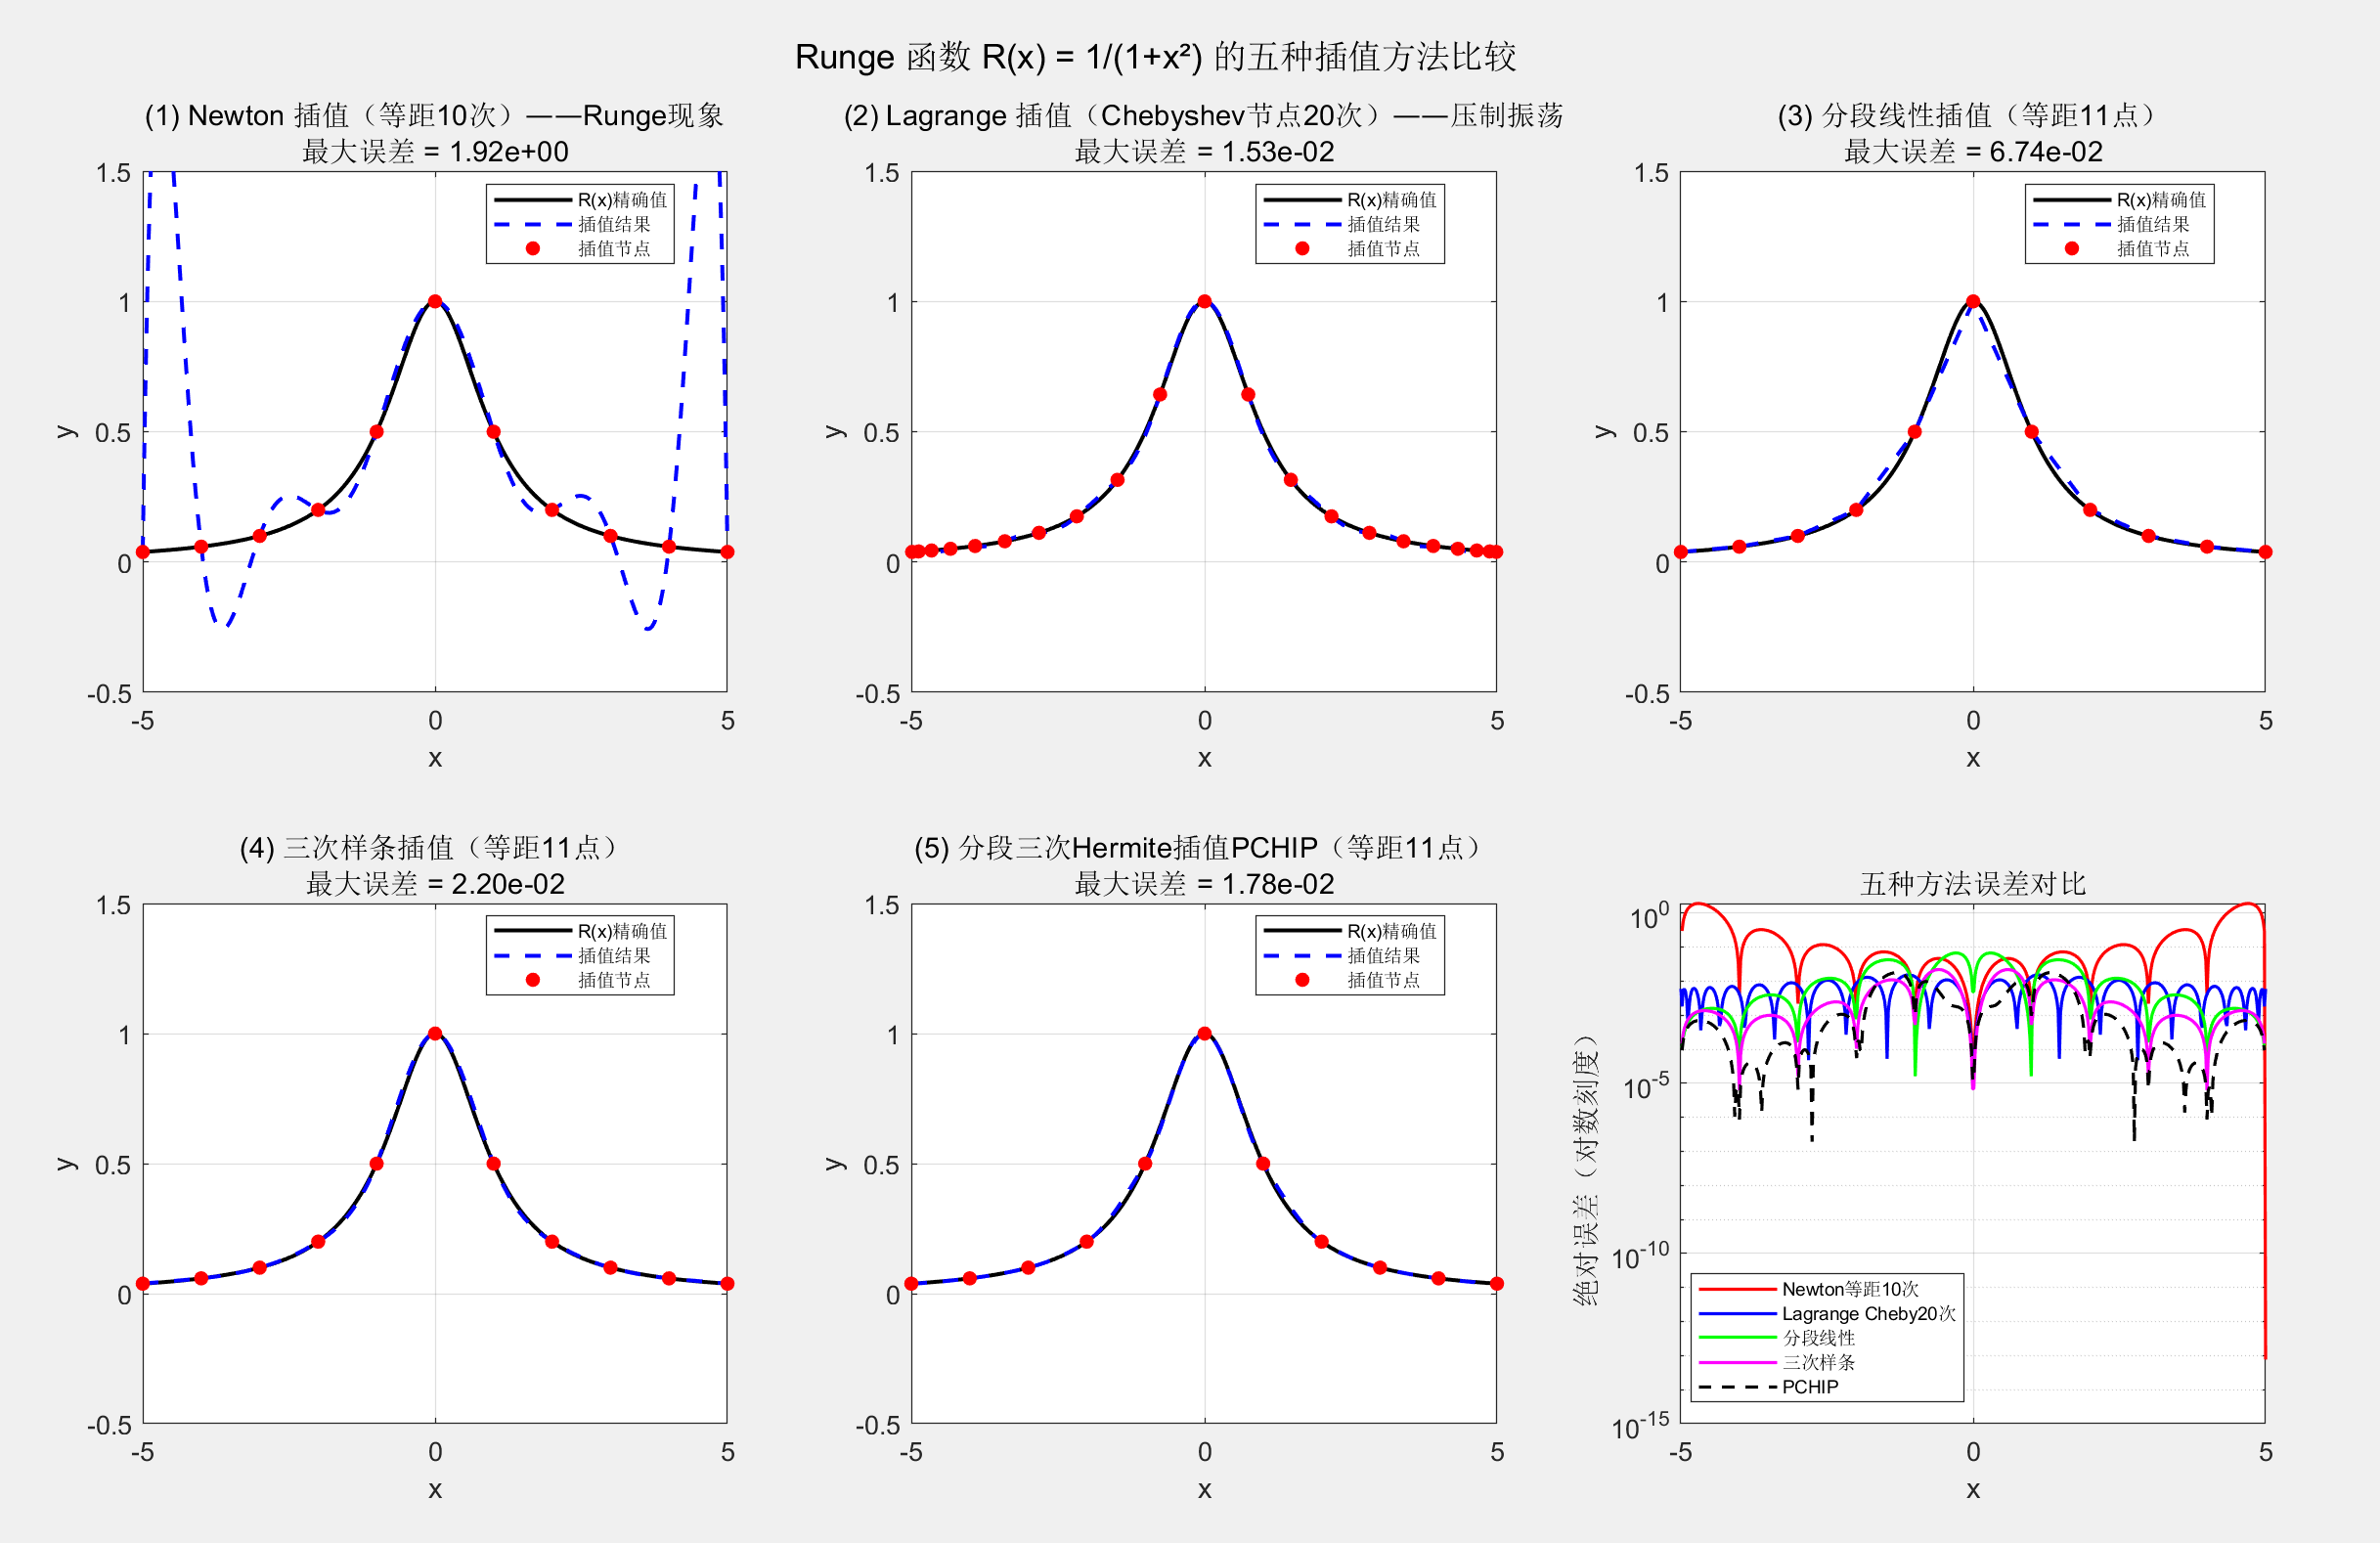
\includegraphics[width=\textwidth]{结果.png}
\caption{Runge 函数 $R(x)=1/(1+x^2)$ 的五种插值方法比较}
\label{fig:result}
\end{figure}

\subsection{各方法分析}

\noindent\textbf{（1）Newton 等距插值——Runge 现象．}
最大误差高达 $1.92$，远大于 $R(x)$ 的值域 $(0,1]$，误差集中在 $x=\pm4$ 至 $\pm5$ 的端部区域，插值曲线在端点附近剧烈振荡，直观上与精确曲线严重背离．这正是 Runge 现象的典型表现：等距高次多项式插值在端点附近不收敛，节点间距均匀导致节点多项式 $\omega_{11}(x)$ 在端部取值极大．

\noindent\textbf{（2）Chebyshev 节点 Lagrange 插值——有效压制振荡．}
最大误差降至 $1.53\times10^{-2}$，比等距 Newton 插值小约 125 倍．Chebyshev 节点在区间两端密集，使节点多项式 $\omega_{21}(x)$ 的最大值达到理论最小，整体误差均匀分布，无端点振荡．尽管多项式次数高达 20 次，逼近效果依然良好，验证了 Chebyshev 节点对压制 Runge 现象的有效性．

\noindent\textbf{（3）分段线性插值——稳定但光滑性差．}
最大误差为 $6.74\times10^{-2}$，是五种方法中等距节点方法误差最大的，但完全无振荡．误差主要来源于 $R(x)$ 曲率较大的峰值区域（$x \approx 0$ 附近），步长 $h=1$ 时线性近似不够精细．插值曲线在节点处出现明显折角，$C^0$ 连续但 $C^1$ 不连续，视觉上不够光滑．

\noindent\textbf{（4）三次样条插值——光滑且精度高．}
最大误差为 $2.20\times10^{-2}$，比分段线性插值误差减小约 3 倍，曲线视觉上非常光滑（$C^2$ 连续）．not-a-knot 边界条件充分利用了内节点处的信息，无需额外的端点导数输入，在同等节点数下精度优于自然样条．

\noindent\textbf{（5）PCHIP——保形性好，精度与样条相近．}
最大误差为 $1.78\times10^{-2}$，略优于三次样条．PCHIP 的导数由局部差商方案确定，保证了单调区间内插值的单调性，不在极值处引入过冲，对 Runge 函数的峰值刻画比三次样条更忠实．光滑性为 $C^1$（低于样条的 $C^2$），但在保形要求下这是合理的代价．

\subsection{综合比较}

\begin{table}[H]
\centering
\caption{五种方法综合特性对比}
\label{tab:compare}
\begin{tabular}{clcccc}
\toprule
编号 & 方法 & 连续性 & 是否保形 & Runge 现象 & 精度（本题）\\
\midrule
(1) & Newton 等距多项式  & $C^\infty$ & 否 & \textbf{有，严重} & 差 \\
(2) & Lagrange Chebyshev & $C^\infty$ & 否 & 无 & 优 \\
(3) & 分段线性           & $C^0$      & 是 & 无 & 一般 \\
(4) & 三次样条           & $C^2$      & 否 & 无 & 良 \\
(5) & PCHIP              & $C^1$      & \textbf{是} & 无 & 良 \\
\bottomrule
\end{tabular}
\end{table}

\section{结论}

\begin{itemize}
  \item \textbf{Runge 现象的根本原因}在于等距节点的节点多项式 $\omega_{n+1}(x)$ 在端点附近无界增长，而非多项式插值本质的问题．采用 Chebyshev 节点可将 $\max|\omega_{n+1}(x)|$ 降至理论最小，彻底消除振荡．
  \item \textbf{Chebyshev 节点 Lagrange 插值}在本题五种方法中误差最小，是全局多项式插值中应对 Runge 现象的标准方案．
  \item \textbf{分段方法（线性/样条/PCHIP）}均为局部方法，天然避免 Runge 现象，适用于节点分布固定（如等距）的场景；三者中三次样条和 PCHIP 精度相近，样条更光滑，PCHIP 更保形．
  \item 实际应用中，若节点可自由选取则优先用 Chebyshev 节点；若节点固定（如等距测量数据）则推荐三次样条或 PCHIP，避免使用高次等距多项式插值．
\end{itemize}

%% ============================================================
%%  附录
%% ============================================================
\clearpage

\section{附录：程序代码}

\begin{lstlisting}[style=matlab, caption={problem1\_interpolation.m（主程序与辅助函数）}]
clear; close all; clc;

R = @(x) 1 ./ (1 + x.^2);          % Runge 函数
x_plot  = linspace(-5, 5, 500);     % 绘图点
y_exact = R(x_plot);                 % 精确值

%% (1) Newton 等距插值（10次）
n1 = 10;
x_nodes1 = linspace(-5, 5, n1+1);
y_nodes1  = R(x_nodes1);
dd1 = newton_divided_diff(x_nodes1, y_nodes1);
y_newton = newton_eval(x_nodes1, dd1, x_plot);

%% (2) Chebyshev 节点 Lagrange 插值（20次）
n2 = 20;  k2 = 0:n2;
x_nodes2 = 5 * cos((2*k2 + 1) / 42 * pi);
y_nodes2  = R(x_nodes2);
y_lagrange = lagrange_eval(x_nodes2, y_nodes2, x_plot);

%% (3) 分段线性插值
y_piecewise_linear = interp1(x_nodes1, y_nodes1, x_plot, 'linear');

%% (4) 三次样条插值（not-a-knot）
y_spline = spline(x_nodes1, y_nodes1, x_plot);

%% (5) 分段三次 Hermite 插值（PCHIP）
y_pchip = pchip(x_nodes1, y_nodes1, x_plot);

%% ---- 局部函数 ----
function dd = newton_divided_diff(x, y)
    n = length(x);  dd = y;
    for j = 1 : n-1
        for k = n : -1 : j+1
            dd(k) = (dd(k) - dd(k-1)) / (x(k) - x(k-j));
        end
    end
end

function y_out = newton_eval(x_nodes, dd, x_query)
    n = length(x_nodes) - 1;
    y_out = dd(n+1) * ones(size(x_query));
    for k = n : -1 : 1
        y_out = y_out .* (x_query - x_nodes(k)) + dd(k);
    end
end

function y_out = lagrange_eval(x_nodes, y_nodes, x_query)
    n = length(x_nodes) - 1;
    m = length(x_query);
    y_out = zeros(1, m);
    for k = 1 : n+1
        lk = ones(1, m);
        for j = 1 : n+1
            if j ~= k
                lk = lk .* (x_query - x_nodes(j)) / (x_nodes(k) - x_nodes(j));
            end
        end
        y_out = y_out + y_nodes(k) * lk;
    end
end
\end{lstlisting}

\end{document}
